% PAGE BUDGET
%
%                          TARGET    CURRENT
%
% Abstract + Introduction  1 3/4     1 3/4
% Preliminaries            3         3 3/4
% Algorithm description    3 1/2     6
% Experiments              2 1/4     2 1/2
% Conclusions              1/3       1/3
% References               1         1 + eps

\documentclass[runningheads]{llncs}
\usepackage{graphicx}
\usepackage{epstopdf}
\usepackage{url}
\usepackage[usenames]{xcolor}
\usepackage[vlined]{algorithm2e}
\usepackage{multirow}
\usepackage{wrapfig}
\usepackage{rotating}
\usepackage{array}
\usepackage{microtype}
\usepackage{cite}
\usepackage[font=small,labelfont=bf,tableposition=top,skip=0pt,justification=raggedright]{caption}
\usepackage{booktabs}

\newcommand{\Jose}[1]{{\color{red} [[JOSE:: #1]]}}
\newcommand{\Leo}[1]{{\color{blue} [[LEO:: #1]]}}
\newcommand{\Meng}[1]{{\color{green} [[MENG:: #1]]}}
\newcommand{\Norbert}[1]{{\color{orange} [[NORBERT:: #1]]}}

\newcommand{\ignore}[1]{}

%* Commands and Environments:  %%%%%%%%%%%%%%%%%%%%%%%%%%%%%%%%%%%%%%%%
%** Macros from JeffreyScottVitter
% Write multichar identifier names using \id in either mathmode or text;
% For ex, $\id{high}(x)$ is an expression using the \id{high} function.
% Use ``\ '' if a space is desired, as in math mode.
\def\id#1{\ensuremath{\mathit{#1}}}
\let\idit=\id
\def\idbf#1{\ensuremath{\mathbf{#1}}}
\def\idrm#1{\ensuremath{\mathrm{#1}}}
\def\idtt#1{\ensuremath{\mathtt{#1}}}
\def\idsf#1{\ensuremath{\mathsf{#1}}}
\def\idcal#1{\ensuremath{\mathcal{#1}}}  % Use with capital letter args only


\def\poly{\idtt{poly}}

\def\access{\idtt{access}}
\def\findopen{\idtt{find\_open}}
\def\findclose{\idtt{find\_close}}
\def\enclose{\idtt{enclose}}
\def\selectopen{\idtt{select\_open}}
\def\selectclose{\idtt{select\_close}}
\def\rankopen{\idtt{rank\_open}}
\def\rankclose{\idtt{rank\_close}}
\def\rmqi{\idtt{rmqi}}
\def\RMQi{\idtt{RMQi}}
\def\child{\idtt{child}}
\def\childrank{\idtt{child\_rank}}
\def\depth{\idtt{depth}}
\def\levelanc{\idtt{level\_anc}}
\def\subtreesize{\idtt{subtree\_size}}
\def\degree{\idtt{degree}}
\def\height{\idtt{height}}
\def\deepestnode{\idtt{deepest\_node}}
\def\lca{\idtt{LCA}}
\def\lmostleaf{\idtt{lmost\_leaf}}
\def\rmostleaf{\idtt{rmost\_leaf}}
\def\leafrank{\idtt{leaf\_rank}}
\def\leafselect{\idtt{leaf\_select}}
\def\prerank{\idtt{pre\_rank}}
\def\postrank{\idtt{post\_select}}
\def\preselect{\idtt{pre\_select}}
\def\postselect{\idtt{post\_select}}
\def\nodeselect{\idtt{node\_select}}
\def\levellmost{\idtt{level\_lmost}}
\def\levelrmost{\idtt{level\_rmost}}
\def\levelsucc{\idtt{level\_succ}}
\def\levelpred{\idtt{level\_pred}}
\def\sumop{\idtt{sum}}
\def\fwdsearch{\idtt{fwd\_search}}
\def\bwdsearch{\idtt{bwd\_search}}
\def\rmq{\idtt{rmq}}
\def\RMQ{\idtt{RMQ}}


\def\rankop{\idtt{rank}}
\def\selop{\idtt{select}}

\newenvironment{myitemize}%
  {\begin{itemize}%
    \setlength{\itemindent}{-.1in}
    \setlength{\itemsep}{\baselineskip}%
    \setlength{\parskip}{-\baselineskip}}%
  {\end{itemize}}

\DeclareMathOperator*{\argmin}{arg\!\min}
\DeclareMathOperator*{\argmax}{arg\!\max}
\newtheorem{lemma}{Lemma}



\begin{document}


\title{Parallel Construction of Succinct Trees\thanks{This work was
    supported by the Emerging Leaders in in the Americas scholarship
    programme, NSERC, and the Canada Research Chairs programme.}}
\titlerunning{Parallel Construction of Succinct Trees}

\author{Leo Ferres\inst{1}
  \and
  Jos\'e Fuentes-Sep\'ulveda\inst{1}
  \and
  Meng He\inst{2}
  \and
  Norbert Zeh\inst{2}}

\authorrunning{Leo Ferres, Jos\'e Fuentes-Sep\'ulveda, Meng He, and Norbert Zeh}

\tocauthor{Leo Ferres, Jos\'e Fuentes-Sep\'ulveda, Meng He, and Norbert Zeh}

\institute{Department of Computer Science, Universidad de Concepci\'on, Chile,\\
  \email{\{lferres,jfuentess\}@udec.cl}
  \and
  Faculty of Computer Science, Dalhousie University, Canada,\\
  \email{\{mhe,nzeh\}@cs.dal.ca}}

\maketitle

\begin{abstract}
  Succinct representations of trees are an elegant solution to
  make large trees fit in main memory while still supporting
  navigational operations in constant time.  However, their construction
  time remains a bottleneck.  We
  introduce a practical parallel algorithm that improves the state of
  the art in succinct tree construction.  Given a tree on $n$ nodes
  stored as a sequence of balanced parentheses, our algorithm
  builds a succinct tree representation in $O(n/p+\lg p)$ time,
  where $p$ is the number of available cores.  The constructed
  representation uses $2n + o(n)$ bits of space and supports a rich
  set of operations in $O(\lg n)$ time.  In experiments using up to
  64 cores and on inputs of different sizes, our algorithm
  achieved good parallel speed-up.
  We also present an
  algorithm that takes $O(n/p + \lg p)$ time to construct the
  balanced parenthesis representation of the input tree required by
  our succinct tree construction algorithm.
\end{abstract}
%

%%%%%%%%%%%%%%%%%%%%%%%%
%%%%% INTRODUCTION %%%%%
%%%%%%%%%%%%%%%%%%%%%%%%

\section{Introduction}
\label{sec:introduction}
Trees lie at the foundation of Computer Science. They are, according
to Knuth, one of the most important ``gifts'' from Computer Science to
mathematics. They are, as such, ubiquitous. We can find trees in every
aspect of everyday computing from the XML/HTML processing of web
browsers to ASTs in compilers. Still, with the advent of very large
amounts of hierarchical data, dealing with huge trees, particularly
their construction for in-memory querying, has become a processing
bottleneck. To solve this, succinct trees...

In this paper, we garner the power of multicore processors to help
with succinct tree construction.



%%%%%%%%%%%%%%%%%%%%%%%%
%%%%% PRELIMINARIES %%%%%
%%%%%%%%%%%%%%%%%%%%%%%%

\section{Preliminaries}
\label{sec:relwork}
\input{relwork}

\subsubsection{Succinct trees.}
\label{subsec:suctrees}
Jacobson~\cite{j1989} first proposed to design succinct data structures. Under the bit probe model, he showed how to represent an ordinal trees on $n$ nodes using $2n+o(n)$ bits, to support the computation of the first child, the next sibling and the parent of any given node in $O(\lg n)$ time. 
Under the word RAM model with $\Theta(\lg n)$ word size, Clark and Munro~\cite{cm1996} showed how to support these operations in constant time. 
Since then, a lot of work has been done on succinct tree representations, to support more navigational operations in trees, to achieve compression, to provide support for update operations, and so on~\cite{mr1997,bdmr1999,grr2004,jss2007,ly2008,hms2012,fm2014,Navarro:2014:FFS:2620785.2601073}. 
All this work created several different ways of representing trees succinctly, and we refer to the article by Raman and Rao~\cite{rr2013} for a thorough survey.

Among the different approaches of representing trees succinctly, we choose to design a parallel algorithm to construct the most recent work by Navarro and Sadakane~\cite{Navarro:2014:FFS:2620785.2601073}, who used the term {\em fully functional} representation to refer to their work. There are several reasons. 
First, their work is the first that achieves a {\em redundancy} of $O(n/\lg^c n)$ bits for any positive constant $c$. 
In succinct data structures, redundancy is defined to be the difference between the actual space cost of the data structure and the information theoretical lower bound, and this quality is of both theoretical and practical importance. 
While all the work mentioned here has a redundancy of $o(n)$ bits, all but the fully functional representation requires a redundancy of $\Omega(n \lg\lg n / \lg n)$ bits. 
Second, the fully functional representation supports a large number of navigational operations in trees. Only the work in \cite{hms2012,fm2014} supports two more operations. 
Table~\ref{tbl:operations} gives the list of operations supported in constant time by the fully functional representation, in which the first group of operators are navigational operators in trees. 
Finally, the most recent experimental studies on succinct trees~\cite{ACNSalenex10} showed an implementation of the fully function representation indeed uses less space than the existing implementations of other succinct tree representations in most cases, and provides faster support for most operations. Thus it is more suitable for most practical applications. 

\begin{table}[t]
\begin{center}
\begin{tabular} {|p{2.4cm}|p{5.2cm}|} \hline
operator name                             &descriptions        \\ \hline
%$\rmqi(i,j)$ /$RMQi(i,j)$             &Position of the minimum/maximum excess value in $P[i..j]$ \\ \hline
$\child(x,i)$                         & $i$th child of node $x$\\
$\child\_rank(x)$                     & Number of left siblings of node $x$\\
$\degree(x)$                          &Degree of node $x$\\
$\depth(x)$                           & Depth of node $x$\\
$\levelanc(x,i)$                      &Ancestor of node $x$ that is $i$ levels above node $x$ \\
$\subtreesize(x)$                     &Number of nodes in the subtree rooted at node $x$ \\
$\height(x)$                          &Height of the subtree rooted at $x$ \\
$\deepestnode(x)$                     &Deepest node in the subtree rooted at node $x$\\
$\lca(x,y)$                           &Lowest common ancestor of nodes $x$ and $y$ \\
$\lmostleaf(x)$ /$\rmostleaf(x)$      &Leftmost/rightmost leaf of the subtree rooted at node $x$\\
$\leafrank(x)$                        &Number of leaves before node $x$ in preorder\\
$\leafselect(i)$                      &$i$th leaf from left to right\\
$\prerank(x)$ /$\postrank(x)$             &Number of nodes preceding node $x$ in preorder/postorder\\
$\preselect$ /$\postselect(i)$            &$i$th node in preorder/postorder\\       
$\levellmost(i)$ /$\levelrmost(i)$       &Leftmost/rightmost node among all the nodes with depth $i$ \\
$\levelsucc(x)$ /$\levelpred(x)$        &Node immediately to the left/right of node $x$ among nodes with depth $i$\\ \hline
$\access(i)$                           &$P[i]$        \\ 
$\findopen(i)$ /$\findclose(i)$       &The matching parenthesis of $P[i]$ \\
$\enclose(i)$                           &Closest enclosing matching parenthesis pair for $P[i]$ \\
$\rankopen(i)$ /$\rankclose(i)$       &Number of opening/closing parentheses in $P[1..i]$\\
$\selectopen(i)$ /$\selectclose(i)$   &The $i$th opening/closing parenthesis\\ \hline
\end{tabular}
\caption{Operations supported by the fully functional representation~\cite{Navarro:2014:FFS:2620785.2601073}, including operations over the corresponding balanced parenthesis sequence.}
\label{tbl:operations}
\end{center}
\end{table}

The fully functional representation is essentially a novel way of representing the balanced parentheses sequence corresponding to a given tree. 
Give a tree $T$ on $n$ nodes, we can generate its corresponding balanced parentheses sequence, $P$, by performing a preorder traversal of $T$. 
During this traversal, we write down an opening parenthesis the first time we visit a node, and a closing parenthesis after visiting all its descendants. 
Thus the length of $P$ is $2n$. 
For the ordinal tree in Figure~\ref{figure:bp}, its parenthesis sequence is $P = ((())((()())(()(())))()())$. 
Table~\ref{tbl:operations} also includes a set of operations over a balanced parenthesis sequence.%, in which the excess value of position $i$ is defined to be the number of opneing parenthesis minums the number of closing parenthesis in $P[1..i]$. 


\begin{figure}[t]
  \centering
  \begin{minipage}{.38\textwidth}
  \centering
  \includegraphics[scale=0.5]{images/bp.pdf}
  \caption{An ordinal tree used as an example.}
  \label{figure:bp}
\end{minipage}%
\hspace{2mm}
  \begin{minipage}{.58\textwidth}
  \centering
  \includegraphics[scale=0.16]{./images/Range-min-max-tree.png}
  \caption{Range min-max tree}
  \label{fig:RangeMinMaxTree} 
\end{minipage}
\end{figure}

%\begin{figure}
%\centering
%\includegraphics[scale=0.5]{images/bp.pdf}
%\caption{An ordinal tree used as an example.}
%\label{figure:bp}
%\end{figure}

The fully function representation is not the first structure that makes use of balanced parentheses to represent trees. 
Munro and Raman~\cite{mr1997} first designed succinct representations of balanced parentheses, and they further used them to represent ordinal trees succinctly, by reducing a set of navigational operations over trees to operations over balanced parentheses. 
They only support a subset of the operations listed in Table~\ref{tbl:operations}. 
To support more operations, researchers designed more auxiliary data structures~\cite{ly2008}. 
Thus, to support the operations in Table~\ref{tbl:operations}, many auxiliary data structures are required, which make the overall data structure overtly complex in both theory and practice. 
The main novelty of Navarro and Sadakane's work~\cite{Navarro:2014:FFS:2620785.2601073} lies in their key strategy of reducing a large set of operations over trees and balanced parentheses to a small set of primitive operations. 
To define these operations, they treated $P$ as a bit vector, by storing a $1$ bit for each opening parenthesis, and a $0$ bit for a closing parenthesis. 
Let $g(\cdot)$ be a function on $[0,1]$. Then, they defined the following primitive operations:

\begin{myitemize}
\item $\sumop(P,g,i,j)\triangleq \sum_{k=i}^jg(P[k])$
\item $\fwdsearch(P,g,i,d)\triangleq \min\{j | j \ge i, \sumop(P,g,i,j) = d\}$
\item $\bwdsearch(P,g,i,d)\triangleq \max\{j | j \le i, \sumop(P,g,j,i) = d\}$
\item $\rmq(P,g,i,j)\triangleq \min\{\sumop(P,g,i,k)| i\le k\le j\}$
\item $\RMQ(P,g,i,j)\triangleq \max\{\sumop(P,g,i,k)| i\le k\le j\}$
\item $\rmqi(P,g,i,j)\triangleq \argmin_{k\in[i,j]}\{\sumop(P,g,i,k)\}$
\item $\RMQi(P,g,i,j)\triangleq \argmax_{k\in[i,j]}\{\sumop(P,g,i,k)\}$
\end{myitemize}

Navarro and Sadakane defined three functions on $[0,1]$: function $\pi$ such that $\pi(1) = 1$ and $\pi(0) = -1$, function $\phi$ such that $\phi(1) = 1$ and $\phi(0) = 0$, and function $\psi$ such that $\psi(1) = 0$ and $\psi(0) = 1$. 
Most of the operations in Table~\ref{tbl:operations} can then be supported using the primitive operations when setting $g(\cdot)$ to be $\pi$, $\phi$ and $\psi$. For example, $\findclose(i)$ can be computed using $\fwdsearch(P,\pi,i,0)$. 
Thus it suffices to support these primitive operations when $g(\cdot) = \pi$, $\phi$ or $\psi$, and a few  navigational operations in trees that can not supported by these primitive operations, which are $\degree$, $\child$, $\childrank$ and the four operations related to leaf nodes in Table~\ref{tbl:operations}. 
To support these operations, a simple data structure called \emph{Range Min-Max tree} ({\tt RMMT}) was designed, supporting operations in logarithmic time when used to represent the entire sequence $P$. 
Then, to achieve constant-time support for operations, $P$ is further partitioned into chunks, each of which is represented by a {\tt RMMT}, which can support operations inside a chunk in constant time when the size of each chunk is small enough. Additional data structures are further constructed to support operations in constant time over the entire sequence $P$. 
% for trees of small size, which is further used to design a representation of large trees. 
%, which can support operations in logarthimic time if used to represent the entire sequence $P$. 
%Then, to achieve constant-time support for operations, $P$ is further partitioned into chuncks, each of which is represented by a {\tt RMTT}, and additional data structures are further constructed. 

\subsubsection{The Range Min-Max Tree}

Let $w$ denote the number of bits in a word. The range min-max tree ({\tt RMMT}) is designed to support the primitive operations for functions $\pi$, $\phi$ and $\psi$. %, when the tree represented has $n = w^c$ nodes for an arbitrary constant $c \ge 1$. % \footnote{Navarro and Sadakane~\cite{Navarro:2014:FFS:2620785.2601073} initially defined a {\tt RMMT} for a tree of polylogarthmic size, which is used as a building block for their solution that achieves constant-time support for operations. They mentioned that, when using this structure for the entire tree, the operations can only be supported in logarithmic time, but the structure is simple and practical, which was the variant implemented and tested in \cite{ACNSalenex10}. As we perform experimental studies on the parallel construction of a {\tt RMMT}, here we directly define it for the entire tree.}.
We first describe how to construct a {\tt RMMT} using the function $\pi$, and later we will show how this can be easily augmented to support the operations for the other two functions. 
Recall that $T$ denotes the input tree on $n$ nodes, and $P$ denotes its balanced parentheses sequence of length $2n$, where $P[i] = 1$ iff the $i$th parenthesis is an opening parenthesis. 
The {\em excess} value at position $i$ of $P$ is defined as $\sumop(P,\pi,0,i) = \sum_{k=0}^{i} \pi(P[k])$. 
Let $E$ be a conceptual array in which $E[i]$ stores the excess value at $P[i]$. 

To introduce the {\tt RMMT}, we first partition $P[1..2n]$ into disjoint chunks of size $s$. We will set a value for $s$ later, and for now, the only restriction is that $s \le w/2$. 
For simplicity, we assume that the length of $P$ is divisible by $s$. 
Each chunk is a leaf of the {\tt RMMT}. The {\tt RMMT} is then defined as a complete $k$-ary tree on these leaves, and we will discuss the choices of the values of $k$ later. %, where $k = \Theta(w/(c\lg w))$. 
The following four conceptual arrays, each of length $O(n/s)$, are defined: $e$, storing the excess value at the last position in each chunk, $m$, storing the minimum excess value inside
each chunk, $M$, storing the maximum excess value inside each
chunk, and $n^*$, storing the number of occurrences of the minimum
value in each chunk. 
Each internal node, $u$, of the {\tt RMMT} also stores in $e[u]$/$m[u]$/$M[u]$ the last/miniumum/maximum of the $e$/$m$/$M$ values stored in its children, and in $n^*[u]$ the total number of times $m[u]$ appears in the chunks corresponding to all the leaf descendants of $u$ in the {\tt RMMT}. 
For the values stored for each internal node and each leaf of the {\tt RMMT}, see Figure~\ref{fig:RangeMinMaxTree} for an example. 
As the {\tt RMMT} is a complete tree, we do not store its structure explicitly. 
Instead, we can simply store the $e$/$m$/$M$/$n^*$ values of its (internal and leaf) nodes in four arrays $e'$/$m'$/$M'$/$n'$, like a heap. 

%\begin{figure}[ht]
%  \centering
%  \includegraphics[scale=0.18]{./images/Range-min-max-tree.png}
%  \caption{Range min-max tree}
%  \label{fig:RangeMinMaxTree} 
%\end{figure}

Combined with a standard succinct data structure technique called {\em table lookup}, a {\tt RMMT} can support the primitive operations for $\pi$, as well as $\degree$, $\child$ and $\childrank$. 
Take the support for $\fwdsearch(P,\pi,i,d)$ for example. 
We first check the chunk containing $P[i]$ to see if the answer is inside the same chunk. 
This can be done in constant time by constructing a universal lookup table whose content does not depend on $P$: For each possible bit vector of length $w/2$, and each of the $w/2$ position in the bit vector, we store the answer of $\fwdsearch(P,\pi,i,d)$ if it can be found inside this bit vector, or $-1$ otherwise. As there are $\sqrt{2^w}$ bit vectors of length $w/2$, this table uses $\sqrt{2^w}\poly(w)$ bits. 
If we find the  answer by performing a table lookup for the chunk containing $P[i]$, then we return. 
Otherwise, we search among the $m$ and $M$ values of the right siblings of the leaf node, $u$, corresponding to this chunk, to find the closest right sibling that contains the answer if the answer is within chunks represented by these siblings. 
If the $m$ and $M$ values (each using $\lceil\lg n\rceil$ bits) of the $k$ children of each internal node can be packed into $O(w)$ bits, i.e., $k \lg n = O(w)$, then we can again construct universal lookup tables for internal nodes to perform this step in constant time. 
We repeat this process until we find a right sibling, $v$, of an ancestor of $u$ whose corresponding substring of $P$ contains the answer. 
We then use a similar idea to descend down the tree starting from $v$ to look for the leaf descendant of $v$ containing the result. 
Thus we can support $\fwdsearch$ in $O(h)$ time where $h$ is the height of the {\tt RMMT}, provided that $k \lg n = O(w)$. 

To support the primitive operations for functions $\phi$ and $\psi$, we can define six arrays $e'_{\phi}$, $m'_{\phi}$, $M'_{\phi}$, $e'_{\psi}$, $m'_{\psi}$ and $M'_{\psi}$ which are similar to $e'$, $m'$ and $M'$ defined for $\pi$ ($n'$ is defined to support $\degree$, $\child$ and $\childrank$ only, and thus we need not define similar arrays for $\phi$ and $\psi$). 
We make use of the following three observations to avoid storing these six arrays explicitly: $\sumop(P, \phi, 0, i)$ and $\sumop(P, \psi, 0, i)$ are nondecreasing, $\sumop(P, \phi, 0, i) + \sumop(P, \psi, 0, i) = i$ and $\sumop(P, \phi, 0, i) - \sumop(P, \psi, 0, i) = \sumop(P, \pi, 0, i)$. 
Thus the each value in these six arrays can be computed in constant time without storing them explicitly. 
We just have to compute universal tables to support operations. 

To support $\leafrank$, $\leafselect$, $\lmostleaf$ and \linebreak $\rmostleaf$, we define a conceptual bit vector $P_1[1..2n]$ in which $P_1[i] = 1$ iff $P[i] = 1$ and $P[i+1] = 0$. 
Hence each $1$ bit in $P_1$ corresponds to a leaf node. 
The support for these operations are then reduced to the support for $\rankop$ and $\selop$ operations on $P_1$ defined as follows: $\rankop(P_1, i)$ returns the number of $1$s in $P_1[1..i]$, and $\selop(P_1, i)$ returns the position of the $i$th occurrence of $1$ in $P_1$. 
For example, we have $\leafrank = \rankop(P_1, i)$. 
The $\rankop$ and $\selop$ operations can be further reduced to the support of $\sumop$ and $\fwdsearch$ for the function $\phi$ on $P_1$, which can be supported using another range min-max tree. 
As any $O(w)$ bits in the sequence $P_1$ can be computed from $P$ in constant time using table lookup, $P_1$ itself need not be stored explicitly, and the cost of storing the information for the internal nodes of this range min-max tree is dominated by the space usage of the range min-max tree for $P$. 

To analyze the space cost, we observe that if we store $P$, $e'$, $m'$, $M'$ and $n'$ explicitly in a straightforward manner, the space cost would be $2n + \frac{k}{k-1} \cdot \frac{n}{s} \cdot \lg n$. 
Navarro and Sadakane commented that if we choose $s = w/2$ and $k = w / \lg n$, we will have a simple structure supporting all the operations in Table~\ref{tbl:operations} in $O(\lg n)$ time. 
However, when the trees are so large that $w = \Theta(\lg n)$, $e'$, $m'$, $M'$ and $n'$ would occupy $O(n)$ bits, and then the overall space is more than a typical succinct tree representation which would use $2n+o(n)$ bits. 
Here we comment that to reduce the overall space cost to $2n+o(n)$ bits, we can set $s = \lceil w\lg n\rceil$ and $k = 2$. With these parameters, looking for a potential answer to a query within a chunk would require $O(\lg n)$ table lookups, and as the height of the tree is $O(\lg n)$, operators can be supported in $O(\lg n)$ time. Note that since the tree is binary when $k = 2$, universal tables are not needed for internal nodes. Thus we have the following lemma:

\begin{lemma}\label{lem:lg}
An ordinal tree and its balanced parentheses sequence can be represented using range min-max trees in $2n + o(n)$ bits, where $n$ is the number of nodes in the tree, to support the operations in Table~\ref{tbl:operations} in $O(\lg n)$ time. 
\end{lemma}

The data structure presented by Lemma~\ref{lem:lg} is practical, and previous experimental studies~\cite{ACNSalenex10} also chose to implement practical versions of {\tt RMMT} that support operations in $O(\lg n)$ time. 
Navarro and Sadakane, however, initially designed {\tt RMMT} in order to use it as a building block in their solution that represents trees succinctly to support operations in constant time. 
They choose a parameter $B = \Theta(\frac{w}{c\lg w})$, and construct a {\tt RMMT} for trees on $(B^c)/2$ nodes, where $c > 3/2$ is an arbitrary constant. 
Note that the length of the parentheses sequence $P$ is now a power of $B$. 
They set $s = k = B$. 
Instead of storing $P$, $e'$, $m'$, $M'$ and $n'$ explicitly, they reduce the space cost by encoding them using the {\em aB-tree}~\cite{Patrascu:2008:SUC:1470582.1470670}. 
When constructed to store $P$, $e'$, $m'$, $M'$ and $n'$, an aB-tree stores $B$ consecutive elements of $P$ in each leaf, and the aB-tree is a complete $B$-ary tree. 
Thus the height of the tree is $c$, the time required to support operations in Table~\ref{tbl:operations} is $O(c) = O(1)$, and the space usage is $2n+2$ bits only. 
Note that universal tables are still required, but if we construct them for all possible bit vectors of length $B$, then their space costs are reduced to $\sqrt{2^w}$ bits. 

\subsubsection{Representing Large Trees}

To support operations in constant time for trees of arbitrary sizes, Navarro and Sadakane partition $P$ into {\em blocks} of length $w^c$. 
Each block may not necessarily store a balanced sequence, but it can still be represented using a {\tt RMMT} in $w^c + 2$ bits.  
The universal tables constructed for different blocks store the same content, so one set of these tables are sufficient. 
The overall space of storing the {\tt RMMT}'s of all these blocks and one set of universal tables is thus $2n + O(n/w^c) + \sqrt{2^w}$ bits. 

2d min-heap

weighted ancestor

rmq

rest

\subsubsection{Dynamic multithreading (DyM) model.}
\label{subsec:dym}
{\em Dynamic multithreading} (DYM) \cite[Chapter 27]{Cormen2009} is a
model of parallel computation which is faithful to several industry standards
such as Intel's CilkPlus (\url{cilkplus.org}) and OpenMP Tasks
(\url{openmp.org/wp}), and Threading Building
Blocks (\url{threadingbuildingblocks.org}).

We will define a {\em multithreaded computation} as a directed acyclic
graph (DAG) $G=(V,E)$, where the set of vertices $V$ are instructions
and $(u,v) \in E$ are dependencies between instructions; whereby in
this case, $u$ must be executed before $v$.\footnote{Notice that the
  RAM model is a subset of the DYM model where the outdegree of every
  vertex $v \in V$ is $\leq 1$.} In order to signal parallel
execution, we will augment sequential pseudocode with three keywords,
{\bf spawn}, {\bf sync} and {\bf parfor}. The {\bf spawn} keyword
signals that the procedure call that it precedes {\em may be} executed
in parallel with the next instruction in the instance that executes
the {\bf spawn}. In turn, the {\bf sync} keyword signals that all
spawned procedures must finish before proceeding with the next
instruction in the stream. Finally, {\bf parfor} is simply ``syntactic
sugar'' for {\bf spawn}'ing and {\bf sync}'ing ranges of a loop
iteration. If a stream of instructions does not contain one of the
above keywords, or a {\bf return} (which implicitly {\bf sync}'s) from
a procedure, we will group these instruction into a single {\em
  strand}. Strands are scheduled onto processors using a {\em
  work-stealing} scheduler, which does the load-balancing of the
computations. Work-stealing schedulers have been proved to be a factor
of 2 away from optimal performance
\cite{Blumofe:1999:SMC:324133.324234}.

To measure the efficiency of our parallel algorithm, we
will use three metrics: the {\em work}, the {\em span} and the number
of processors. In accordance to the parallel literature, we will
subscript running times by $P$, so $T_P$ is the running time of an
algorithm on $P$ processors. The {\em work} is the total running time
taken by all (unit-time) strands when executing on a {\em single}
processor (i.e., $T_1$),\footnote{Notice, again, that analyzing the
  work amounts to finding the running time of the serial algorithm
  using the RAM model.} while the {\em span}, denoted as $T_\infty$,
is the {\em critical path} (the longest path) of $G$. In this work,
we are interested in speeding up the succinct tree construction and finding
out the upper bounds of this speedup. To measure this, we will define
{\em speedup} as $T_1/T_P = O(P)$, where linear speedup $T_1/T_P =
\Theta(P)$, is the goal. We also define {\em parallelism} as the ratio
$T_1/T_{\infty}$, the maximum theoretical speedup that can be achieved
on {\em any} number of processors.

\section{A Parallel Algorithm for Succinct Tree Construction}
\label{sec:multicoreST}
We now propose a parallel algorithm that constructs the {\tt RMMT} of
a given tree. Our algorithm, called the \emph{Parallel Succinct Tree
  Algorithm} ({\tt PSTA}), has as input a tree on $n$ nodes stored in
the form of a sequence of balanced parentheses, $P$, of size $2n$.  In
practice, it is common to store, in secondary storage, an ordinal tree
in the form of a sequence of balanced parenthesis; this scheme is
often called the ``folklore'' encoding.  Hence we make such an
assumption on the input.  For trees whose folklore encoding is not
directly available, we describe, in
Appendix~\ref{subsec:parenthesesAlgorithm}, an algorithm that can
compute such an encoding in parallel.  Our algorithm requires a model
that supports parallelism and can manipulate $w$ bits in $O(1)$ time,
where $w$ is the number of bits in a word. DYM meets these
criteria. Additionally, we consider the overhead (in space and time)
imposed by the scheduling of cores to be negligible. This is
guaranteed by the results of \cite{Blumofe:1999:SMC:324133.324234},
and in fact the number of available processing units in current
systems is generally much smaller than the input size $n$, so this
cost is also negligible in practice.

\begin{figure}[t!]
\begin{minipage}[t]{.50\textwidth}
  \vspace{0pt}
  \begin{algorithm}[H]
\small
\SetVlineSkip{-2cm}
  % keywords
  \SetKwInOut{Input}{Input}
  \SetKwInOut{output}{output}
  \SetKwFor{PFor}{parfor}{do}{end}
  \LinesNumbered
  \SetAlgoNoEnd
  \DontPrintSemicolon
  % I/o
  \Input{$P$, $s$, $threads$}
  \output{$e^{\prime}, m^{\prime}, M^{\prime}, n^{\prime}$ and universal tables ({\tt RMMT})}  \BlankLine% \SetAlgoNoLine
  % algorithm
  $o$ = $\lceil 2n/s \rceil-1$\tcp*[h]{\# internal nodes}\;
  $e^{\prime}$ = array of size $\lceil 2n/s \rceil$\;
  $m^{\prime}, M^{\prime}, n^{\prime}$ = arrays of size $\lceil 2n/s \rceil + o$\;
  $ct$ = $\lceil 2n/s \rceil/threads$\;%\tcp*[h]{Chunks per thread}\;
  \PFor{$t\leftarrow 0$ \KwTo $threads-1$}{
	  $e^{\prime}_t, m^{\prime}_t, M^{\prime}_t, n^{\prime}_t$ = $0$\;

	  \For{$chk \leftarrow 0$ \KwTo $ct-1$}{
		  $low$ = $t*ct*s+chk*s$\;
		  $up$ = $low+s$\;
		  \For{$par \leftarrow low$ \KwTo $up-1$}{
			$e^{\prime}_t$ += $2*P[par]-1$\;
%		  	\eIf{$P[par]$ is $closed$}{
%		  		$e^{\prime}_t$ -= $1$\;
%		  	}
%		    {
%		  		$e^{\prime}_t$ += $1$\;
%		    }
		    \uIf{$e^{\prime}_t < m^{\prime}_t$}{
				$m^{\prime}_t$ = $e^{\prime}_t$;
				$n^{\prime}_t$ = $1$
			}
			\uElseIf{$e^{\prime}_t == m^{\prime}_t$}{
				$n^{\prime}_t$ += $1$\;
			}
			\uElseIf{$e^{\prime}_t > M^{\prime}_t$}{
				$M^{\prime}_t$ = $e^{\prime}_t$\;
			}
		  }
		  $e^{\prime}[t*ct+chk]$ = $e^{\prime}_t$\;
		  $m^{\prime}[t*ct+chk+o]$ = $m^{\prime}_t$\;
		  $M^{\prime}[t*ct+chk+o]$ = $M^{\prime}_t$\;
		  $n^{\prime}[t*ct+chk+o]$ = $n^{\prime}_t$\;		  
	  }
  }
  \BlankLine
  $parallel\_prefix\_sum(e^{\prime}, ct)$\;
%  \For{$t \leftarrow 1$ \KwTo $threads-1$}{
%		$e^{\prime}[(t+1)*ct-1]$ += $e^{\prime}[t*ct-1]$\;
 % }
  \BlankLine
  \PFor{$t\leftarrow 1$ \KwTo $threads-1$}{
	  \For{$chk \leftarrow 0$ \KwTo $ct-1$}{
	  	\If{$chk < ct-1$}{
	  	  $e^{\prime}[t*ct+chk]$ += $e^{\prime}[t*ct-1]$\;
	  	}
  	  	$m^{\prime}[t*ct+chk+o]$ += $e^{\prime}[t*ct-1]$\;
  	  	$M^{\prime}[t*ct+chk+o]$ += $e^{\prime}[t*ct-1]$\;
	  }
  }
%  \Return{$WT$}\;
  \caption{{\tt PSTA} (part I)}
  \label{algo:PSTA1}
  \end{algorithm}
\end{minipage}%
%hfill
\begin{minipage}[t]{.51\textwidth}
  \vspace{0pt}
  \begin{algorithm}[H]
\small
\SetVlineSkip{-2cm}
  \SetKwFor{PFor}{parfor}{do}{end}
  \LinesNumbered
  \SetAlgoNoEnd
  \DontPrintSemicolon
  \SetAlgoLined
  \setcounter{AlgoLine}{1}\ShowLn
  $lvl$ = $\lceil \lg threads \rceil$\;
  \setcounter{AlgoLine}{2}\ShowLn
  \PFor{$st\leftarrow 0$ \KwTo $2^{lvl}-1$}{
      \setcounter{AlgoLine}{3}\ShowLn
	  \For{$l\leftarrow \lceil\lg (2n/s)\rceil-1$ \KwTo $lvl$}{
          \setcounter{AlgoLine}{4}\ShowLn
		  \For{$d\leftarrow 0$ \KwTo $2^{l-lvl}-1$}{
            \setcounter{AlgoLine}{5}\ShowLn
		  	$i$ = $d + 2^{l} - 1 +st*2^{l-lvl}$\;
          \setcounter{AlgoLine}{6}\ShowLn
			$concat(i,m^{\prime},M^{\prime},n^{\prime})$\;	  	
		  }
	  }
  }
  \BlankLine
  \setcounter{AlgoLine}{7}\ShowLn
  \For{$l\leftarrow lvl-1$ \KwTo $0$}{
	  \setcounter{AlgoLine}{8}\ShowLn
	  \PFor{$d\leftarrow 0$ \KwTo $2^{l}-1$}{
        \setcounter{AlgoLine}{9}\ShowLn
	  	$i$ = $d + 2^{l}-1$\;
        \setcounter{AlgoLine}{10}\ShowLn
		$concat(i,m^{\prime},M^{\prime},n^{\prime})$\;	  	
	  }
  }
  \caption{{\tt PSTA} (part II)}
  \label{algo:PSTA2}
	  \end{algorithm}
  \begin{algorithm}[H]
\small
  \SetKwFor{PFor}{parfor}{do}{end}
  \LinesNumbered
  \SetAlgoNoEnd
  \DontPrintSemicolon
  \setcounter{AlgoLine}{1}\ShowLn
  \PFor{$x\leftarrow -w$ \KwTo $w-1$}{
      \setcounter{AlgoLine}{2}\ShowLn
      \PFor{$y\leftarrow 0$ \KwTo $\sqrt{2^{w}}-1$}{
          \setcounter{AlgoLine}{3}\ShowLn
          $i\leftarrow ((x+w) << w)$ OR $w$\;
          \setcounter{AlgoLine}{4}\ShowLn
          $near\_fwd\_pos[i] = w$\;
          \setcounter{AlgoLine}{5}\ShowLn
          $p, excess$ = $0$\;
          \setcounter{AlgoLine}{6}\ShowLn
          \Repeat{$p\geq w$}{
              \setcounter{AlgoLine}{7}\ShowLn
              $excess$ += $1-2*((y$ AND $(1 << p)) == 0)$\;
              \setcounter{AlgoLine}{8}\ShowLn
              \If{$excess == x$}{
                  \setcounter{AlgoLine}{9}\ShowLn
                  $near\_fwd\_pos[i] = p$\;
                  \setcounter{AlgoLine}{10}\ShowLn
                  $break$\;
              }
              \setcounter{AlgoLine}{11}\ShowLn
              $p$ += $1$\;
          }
      }
  }
  \caption{{\tt PSTA} (part III)}
  \label{algo:PSTA3}
  \end{algorithm}
\begin{function}[H]
 \SetKwInOut{Input}{Input}
  \SetKwInOut{output}{output}
  \SetKwFor{PFor}{parfor}{do}{end}
  \LinesNumbered
  \SetAlgoNoEnd
  \DontPrintSemicolon
  \SetAlgoLined
  % I/o
  \Input{$i$, $m^{\prime}$, $M^{\prime}$, $n^{\prime}$}
  \BlankLine% \SetAlgoNoLine
   $m^{\prime}[i]$ = $min(m^{\prime}[2i+1], m^{\prime}[2i+2])$\;
   $M^{\prime}[i]$ = $max(M^{\prime}[2i+1], M^{\prime}[2i+2])$\;
   $n^{\prime}[i]$ = $n^{\prime}[2i+1]$\;
   \uIf{$m^{\prime}[2i+1]>m^{\prime}[2i+2]$}{
	   $n^{\prime}[i]$ = $n^{\prime}[2i+2]$\;
    }\uElseIf{$m^{\prime}[2i+1]==m^{\prime}[2i+2]$}{
	  $n^{\prime}[i]$ += $n^{\prime}[2i+2]$\;
	}
  \caption{concat()}
  \label{func:concat}
\end{function}
\end{minipage}
\caption{The pseudocode of {\tt PSTA}.}
\label{fig:psta}
\normalsize
\vspace{-20pt}
\end{figure}

Before describing the {\tt PSTA} algorithm, we observe
that, the entries in $e'$ that correspond to the internal nodes of the
{\tt RMMT} need not be stored explicitly.  This is because the entry
of $e'$ corresponding to an internal node is equal to the entry that
corresponds to the last leaf descendant of this node; as the {\tt
  RMMT} is complete, we can easily locate such a leaf in constant
time.  Thus, in the description of our algorithm, we treat $e'$ as an
array of length $\lceil 2n / s\rceil$, in which each entry corresponds
to a leaf.  Our algorithm then consists of three phases. In the first
phase, it computes the leaves of the {\tt RMMT}, i.e., the array $e'$,
as well as the entries of $m^{\prime}$, $M^{\prime}$ and $n^{\prime}$
that correspond to the leaves of the {\tt RMMT}.  In the second phase,
the algorithm computes the internal nodes of the {\tt RMMT}, i.e., the
remaining entries of $m^{\prime}$, $M^{\prime}$ and $n^{\prime}$.
Finally, in the last phase, it computes the universal tables used in
the {\tt RMMT} in parallel.  In our discussions, we assume that the
input of our algorithm includes $P$, a parentheses sequence of size
$2n$; $s$, the size of each chunk; and $threads$, the total numbers of
available threads.  The pseudocode of the sequential version of our
algorithms can be obtained by replacing {\bf parfor} instructions by
sequential {\bf for} instructions in the pseudocode shown in
Figure~\ref{fig:psta}.

Algorithm \ref{algo:PSTA1} presents the pseudocode for computing the
leaves of the {\tt RMMT}.  Recall that the size of array $e^{\prime}$
is the number of leaves in the {\tt RMMT} (line 2), and the size of
arrays $m^{\prime}$, $M^{\prime}$ and $n^{\prime}$ is the total number
of nodes in the {\tt RMMT}, i.e., $2\lceil 2n/s \rceil-1$ (lines 1 and
3).  In this algorithm, we first assign the same number of consecutive
chunks to each core.  The number $ct$ of chunks assigned to each core
is computed as $\lceil 2n / s\rceil / threads $ (line 4); we assume
that $\lceil 2n / s\rceil$ is divisible by $threads$ for simplicity.
The chunks assigned to each core forms a contiguous subsequence of
$P$, and we compute in parallel the {\em local} excess value of the
last position in each chunk by letting each core loop through the
subsequence assigned to it.  Here the local excess value of a position
$i$ is defined to be $\sumop(P,\pi,j,i)$, where $j$ is the index in
$P$ that corresponds to the starting position of the subsequence
assigned to the core that computes the local excess value at position
$i$.  These local excess values are stored in $e'$.  During this
process, we also compute the minimum and maximum values of the local
excess values in each chunk, and store them in the corresponding
entries $m$ and $M'$, respectively.  During this process, we can
correctly compute the entries of $n'$ that correspond to leaves.
Lines 4 to 21 show the computation.
% , in which each thread computes the excess value of $ct$ consecutive
% chunks by walking through them, following the above equation to
% compute local excess values.  Each time an opening parenthesis
% appears in a chunk, the thread increments the current local excess
% value that it is maintaining, and decrements the value otherwise
% (lines 11 to 14).  Immediately after the local excess changes, it is
% necessary to verify if the maximum, minimum and number of minimum
% values also change (lines 15 to 21). When a chunk is completed, the
% local excess and its associated values are stored in the arrays
% $e^{\prime}$, $m^{\prime}$, $M^{\prime}$ and $n^{\prime}$ (lines 22
% to 25).

The arrays $e'$, $m'$ and $M'$ now store the local excess values for
the leaf nodes of the {\tt RMMT}, and we next update them to store the
corresponding global excess values in $P$.  To do this, we first
update the excess value of the last position of the subsequence
assigned to each core.  We observe that for the $i$th core, the global
excess value of the last position in its subsequence is equal to the
sum of the local excess values of the last positions in the
subsequences assigned to the first $i$ cores.  Therefore, we can use a
parallel prefix sum algorithm~\cite{Helman2001265} to update all these
values (line 22).  Each process can now then update the remaining
excess, minimum and maximum values in parallel, by making use of the
excess value of the last position of the subsequence assigned to the
previous core (lines 23 to 28).
% Note that the prefix sum algorithm computes the prefix sums over
% only $p$ values.

Algorithm \ref{algo:PSTA2} shows the computation of the internal
nodes.  Here, we first compute the closest level, $lvl$, to the root
that has at least $p$ nodes (line 1).  Note that we number the levels
incrementally starting from the root, which is at level $0$.  Then for
each node at level $lvl$, we assign the subtree rooted at it to a
core.  This core computes the entries of $m$, $M'$ and $n'$ that
correspond to each node in this subtree, by processing the entries of
$m$, $M'$ and $n'$ corresponding to its two children (lines 2-6). Line
6 calls $concat$, whose pseudocode is also given.  Notice that one
core could compute more than one subtree and those subtrees may be
non-consecutive. With a scheduler that balances the work, such as a
work-stealing scheduler, cores have a similar workload.  Finally, for
each of the remaining levels (levels $lvl-1, lvl-2, \ldots 0$), the
algorithm computes the entries of $m$, $M'$ and $n'$ that correspond
to the nodes at each level in parallel (lines 7-10).

In the last phase of {\tt PSTA}, Algorithm \ref{algo:PSTA3} shows the
computation of universal tables.  As each entry in a universal table
can be computed independently, we can easily compute them in parallel.
To simplify the explanation, Algorithm \ref{algo:PSTA3} just shows the
computation of one universal table, $near\_fwd\_pos$, which is the one
used to support the {\fwdsearch} operation (its content is described
in Section~\ref{subsec:suctrees}). The same algorithm can be applied
to the other tables.
%
%All of these tables do not depend on the input, except for the
%number of available threads.
%
%
%The {\tt RMMT} is constructed over $P$, partitioning $P$ in disjoint
%chunks of size $s$. Considering those chunks, the construction of the
%{\tt RMMT} is based in the computation of different arrays of size
%$O(\frac{N}{s})$. Such arrays are $e^{\prime}$, saving the final
%excess of each chunk, $m^{\prime}$, saving the minimum excess value of
%each chunk, $M^{\prime}$, saving the maximum excess value of each
%chunk and $n^{\prime}$, saving the number of ocurrences of the minimum
%value of each chunk. As a reminder, the excess value at position $i$
%is:
%\begin{equation}
%  \displaystyle E[i] = \sum_{k=0}^{i} \pi(P[k])
%  \label{eq:excess}
%\end{equation}
%
%where $\pi(``(") = 1$ and $\pi(``)") = -1$. See Figure
%\ref{fig:RangeMinMaxTree} as an example of {\tt RMMT}, with $s=3$ and
%$k=3$.
%
%\begin{figure}[ht]
%  \centering
%  \includegraphics[scale=0.18]{./images/Range-min-max-tree.png}
%  \caption{Range min-max tree}
%  \label{fig:RangeMinMaxTree} 
%\end{figure}
%
%The first step of {\tt PSTA} is to compute the arrays $e^{\prime}$,
%$m^{\prime}$, $M^{\prime}$ and $n^{\prime}$ in parallel. Since
%$e^{\prime}$ just saves the last excess value of each chunk, which is
%a sum, {\tt PSTA} needs to apply a parallel prefix sum
%algorithm. Computing the last element of $e^{\prime}$, at position
%$\frac{2n}{s}-1$, we indirectly compute the rest of the elements of
%$e^{\prime}$. We adapted the algorithm in \cite{Helman2001265} for
%this context, computing $e^{\prime}$ in $O(\frac{n}{p}+\lg p)$ time, using
%$p$ threads. Note that we do not need to compute more elements of
%$e^{\prime}$ to the internal nodes of the {\tt RMMT}. The memory used
%in construction time are bounded by $O(n\lg(n))$ bits.
%
%To compute $m^{\prime}$, let's assume, without loss of generality,
%that $p = k^{i}$, where $k$ is the arity
%of the internal nodes in the {\tt RMMT} and $i > 0$. {\tt PSTA}
%assigns one thread per sub-tree of size $O(\frac{n}{sp})$, at level
%$i$. So, it is possible to compute the $m^{\prime}$ values in all
%sub-trees, in parallel, in $O(\frac{n}{sp}k)$ time. Then, for the
%rest $O(p)$ nodes in the top of the tree, we compute the corresponding
%minimum values in $O(k\lg_{k} p)$ time, computing each level in $O(k)$
%time, just looking the $k$ values on the previous level using one
%thread per vertex. If we consider $s$ and $k$ as constants, we can compute
%$m^{\prime}$ in
%$O(\frac{n}{sp}k + \lg p) = O(\frac{n}{p}+\lg p)$ time,
%using $O(n\lg(n))$ bits in construction time and in the
%final array. Note that this solution makes sense considering that
%$p\ll N$. Figure \ref{fig:min-max-array} illustrates the solution
%explained here. We can compute $M^{\prime}$ and $n^{\prime}$ in the
%same way, obtaining the same complexity.
%
%\begin{figure}[t]
%  \centering
%  \includegraphics[scale=0.28]{./images/Min-Max-array.png}
%  \caption{Computation of $m^{\prime}$ and $M^{\prime}$}
%  \label{fig:min-max-array} 
%\end{figure}
%
%In addition to the arrays, the construction of the {\tt RMMT} involves
%the computation of \emph{universal tables}.
%The universal tables are
%used to support \emph{fwd\_search}($\bullet$),
%\emph{bwd\_search}($\bullet$), \emph{rmqi}($\bullet$),
%\emph{RMQi}($\bullet$), \emph{degree}($\bullet$) and
%\emph{child}($\bullet$) queries.
%We can divide
%universal tables into two types: those that depend on the leaves of
%the {\tt RMMT} and those that depend on the internal nodes. In the
%first case, we can compute each universal table in parallel assigning
%one processor per leaf or chunk, which allows to compute different
%parts of the table at the same time. For the second kind of tables, we
%can assign one processor per internal node. Such processor computes
%the section corresponding to that internal node in the universal
%table. In that way, since computing the universal tables sequentially
%has a complexity of $O(\sqrt{2^{w}}poly(w))$ time according to
%\cite{Navarro:2014:FFS:2620785.2601073}, we can compute those
%universal tables in $\displaystyle O(\sqrt{2^{w}}poly(w)/p)$,
%using $p$ processors.
%
%To reduce the space used by the {\tt RMMT}, Sadakane and Nava\-rro used
%the \emph{aB-tree}. As the {\tt RMMT} and aB-tree are both complete trees, we can apply a
%construction as that shown in Figure \ref{fig:min-max-array} to
%construct the aB-tree. With respect to the universal tables needed in
%the aB-tree, they can be computed following the same strategy
%explained previously, but now with size $O(\sqrt{2^{w}})$
%bits.


\subsubsection{Theoretical Analysis.}
\label{subsec:theoreticalAnalysis}
The {\tt PSTA} algorithm is shown in Algorithm \ref{algo:PSTA1}, \ref{algo:PSTA2} and \ref{algo:PSTA3}. Algorithm \ref{algo:PSTA1} shows the computation of the leaves of the {\tt RMMT}, Algorithm \ref{algo:PSTA2} shows the computation of the internal nodes  of the {\tt RMMT} and finally Algorithm \ref{algo:PSTA3} shows the computation of the universal tables. The sequential version of {\tt PSTA} can be obtained by replacing {\bf parfor} instruction with sequential {\bf for} instructions. The algorithm takes as input a parentheses sequence $P$, the arity $k$ of the internal nodes in the {\tt RMMT}, the size of each chunk $s$ and the total numbers of available threads. In the sequence $P$, opened-parenthesis and closed-parenthesis are coded by $1$ and $0$, respectively. The output is the {\tt RMMT} represented by its arrays $e^{\prime}$, $m^{\prime}$, $M^{\prime}$, $n^{\prime}$ and universal tables, used to support queries in constant time.

\begin{algorithm}[t]
\small
\SetVlineSkip{-2cm}
  % keywords
  \SetKwInOut{Input}{Input}
  \SetKwInOut{output}{output}
  \SetKwFor{PFor}{parfor}{do}{end}
  \LinesNumbered
  \SetAlgoNoEnd
  \DontPrintSemicolon
  % I/o
  \Input{Parentheses sequence $P$, $k$, $s$, $num\_threads$}
  \output{$e^{\prime}, m^{\prime}, M^{\prime}, n^{\prime}$ and universal tables ({\tt RMMT})}
  \BlankLine% \SetAlgoNoLine
  % algorithm
  $o$ = $\frac{\lceil |P|/s \rceil-1}{k-1}$\tcp*[h]{Internal nodes of the RMMT}\;
  $e^{\prime}$ = array of size $\lceil |P|/s \rceil$\;
  $m^{\prime}, M^{\prime}, n^{\prime}$ = arrays of size $\lceil |P|/s \rceil + o$\;
  $ct$ = $\lceil |P|/s \rceil/num\_threads$\tcp*[h]{Chunks per thread}\;
  \PFor{$t\leftarrow 0$ \KwTo $num\_threads-1$}{
	  $partial\_excess, local\_min$ = $0$\;
	  $local\_max, num\_mins$ = $0$\;
	  
	  \For{$chunk \leftarrow 0$ \KwTo $ct$}{
		  $llimit$ = $t*ct*s+chunk*s$\;
		  $ulimit$ = $llimit+s$\;
	  	
		  \For{$par \leftarrow llimit$ \KwTo $ulimit$}{
		  	\eIf{$P[par]$ is $closed$}{
		  		$partial\_excess$ -= $1$\;
		  	}
		    {
		  		$partial\_excess$ += $1$\;
		    }
		    
		    \uIf{$partial\_excess < local\_min$}{
				$local\_min$ = $partial\_excess$\;
				$num\_mins$ = $1$
			}
			\uElseIf{$partial\_excess == local\_min$}{
				$num\_mins$ += $1$\;
			}
			\uElseIf{$partial\_excess > local\_max$}{
				$local\_max$ = $partial\_excess$\;
			}
		  }
		  $e^{\prime}[t*ct+chunk]$ = $local\_excess$\;
		  $m^{\prime}[t*ct+chunk+o]$ = $local\_min$\;
		  $M^{\prime}[t*ct+chunk+o]$ = $local\_max$\;
		  $n^{\prime}[t*ct+chunk+o]$ = $num\_mins$\;		  
	  }
  }
  \BlankLine
  \For{$t \leftarrow 1$ \KwTo $num\_threads-1$}{
		$e^{\prime}[(t+1)*ct]$ += $e^{\prime}[t*ct-1]$\;
  }
  \BlankLine
  \PFor{$t\leftarrow 1$ \KwTo $num\_threads$}{
	  \For{$chunk \leftarrow 0$ \KwTo $ct$}{
	  	\If{$t == num\_threads-1$ OR $chunk < ct-1$}{
	  	  $e^{\prime}[t*ct+chunk]$ += $e^{\prime}[t*ct-1]$\;
	  	}
  	  	$m^{\prime}[t*ct+chunk+o]$ += $e^{\prime}[t*ct-1]$\;
  	  	$M^{\prime}[t*ct+chunk+o]$ += $e^{\prime}[t*ct-1]$\;
	  }
  }


%  \Return{$WT$}\;

  \caption{{\tt PSTA} (part I)}
  \label{algo:PSTA1}
\end{algorithm}
\normalsize

	Let's analyze the Algorithm \ref{algo:PSTA1}. Since the {\tt RMMT} can be seen as a complete tree of arity $k$, it is easy to calculate the size of the arrays $e^{\prime}$, $m^{\prime}$, $M^{\prime}$ and $n^{\prime}$. The size of array $e^{\prime}$ is the number of leaves of the {\tt RMMT} (line 2). The size of arrays $m^{\prime}$, $M^{\prime}$ and $n^{\prime}$ is equal to the total number of nodes of the {\tt RMMT}, that is, $\frac{\lceil |P|/s \rceil-1}{k-1} + \lceil |P|/s \rceil$ (lines 1 and 3). Lines 4 to 26 shows the computation of partial excess values in parallel. The first step is to compute the number of chunks that each thread has to process (line 4). Then, in parallel, each thread computes the excess value of $ct$ consecutive chunks, following the Equation \ref{eq:excess}. In each chunk, the thread increases by one the partial excess value each time that a open parenthesis appears, and decreases by one in other case (lines 12 to 15). Immediately after the partial excess changes, it is necessary to verify if the maximum, minimum and number of minimum values change, too (lines 16 to 22). When a chunk is completed, the local excess and its associated values are stored in the arrays $e^{\prime}$, $m^{\prime}$, $M^{\prime}$ and $n^{\prime}$ (lines 23 to 26). After a thread finishes its chunks, it is necessary to complement its local excess values considering the local values of previous threads. To do that, first we update sequentially the final excess value of each thread (lines 27 and 28). Those excess values do not need to be changed again. Now, thanks to the final excess value of each thread is updated, each thread can update the other excess, minimum and maximum values in parallel (lines 29 to 34). At this point, {\tt PSTA} has computed all the leaves of the {\tt RMMT} in parallel.

\begin{algorithm}[t]
\small
\SetVlineSkip{-2cm}
  % keywords
  \SetKwInOut{Input}{Input}
  \SetKwInOut{output}{output}
  \SetKwFor{PFor}{parfor}{do}{end}
  \LinesNumbered
  \SetAlgoNoEnd
  \DontPrintSemicolon
  % I/o
  \Input{Parentheses sequence $P$, $k$, $s$, $num\_threads$}
  \output{$e^{\prime}, m^{\prime}, M^{\prime}, n^{\prime}$ and universal tables ({\tt RMMT})}
  \BlankLine% \SetAlgoNoLine
  % algorithm

  $level$ = $\lceil \log_{k}num\_threads \rceil$\;
  \PFor{$subtree\leftarrow 0$ \KwTo $k^{level}$}{
	  \For{$l\leftarrow \log_{k}(\lceil |P|/s \rceil-1)$ \KwTo $level$}{
		  \For{$node\leftarrow 0$ \KwTo $k^{l-level}$}{
		  	$pos$ = $node + k^{l} - 1 +subtree*k^{l-level}$\;
			\For{$child\leftarrow pos*k+1$ \KwTo $(pos+1)*k$}{
				\tcp*[h]{first time}\;
			  	\eIf{$child == pos*k+1$}{
				  $m^{\prime}[pos]$ = $m^{\prime}[child]$\;
				  $M^{\prime}[pos]$ = $M^{\prime}[child]$\;
				  $n^{\prime}[pos]$ = $n^{\prime}[child]$\;					
			  	}
			    	{
				    \uIf{$m^{\prime}[child] < m^{\prime}[pos]$}{
						$m^{\prime}[pos]$ = $m^{\prime}[child]$\;
						$n^{\prime}[pos]$ = $n^{\prime}[child]$\;
					}
					\uElseIf{$m^{\prime}[child] == m^{\prime}[pos]$}{
						$n^{\prime}[pos]$ += $n^{\prime}[child]$\;
					}
					\uElseIf{$M^{\prime}[child] > M^{\prime}[pos]$}{
						$M^{\prime}[pos]$ = $M^{\prime}[child]$\;
					}
		    		}
			}		  	
		  }
	  }
  }
  \BlankLine
  \For{$l\leftarrow level-1$ \KwTo $0$}{
	  \PFor{$node\leftarrow 0$ \KwTo $k^{l}$}{
	  	$pos$ = $node + \frac{k^{l}-1}{k-1}$\;
		\For{$child\leftarrow pos*k+1$ \KwTo $(pos+1)*k$}{
			\tcp*[h]{first time}\;
		  	\eIf{$child == pos*k+1$}{
			  $m^{\prime}[pos]$ = $m^{\prime}[child]$\;
			  $M^{\prime}[pos]$ = $M^{\prime}[child]$\;
			  $n^{\prime}[pos]$ = $n^{\prime}[child]$\;					
		  	}
		    	{
			    \uIf{$m^{\prime}[child] < m^{\prime}[pos]$}{
					$m^{\prime}[pos]$ = $m^{\prime}[child]$\;
					$n^{\prime}[pos]$ = $n^{\prime}[child]$\;
				}
				\uElseIf{$m^{\prime}[child] == m^{\prime}[pos]$}{
					$n^{\prime}[pos]$ += $n^{\prime}[child]$\;
				}
				\uElseIf{$M^{\prime}[child] > M^{\prime}[pos]$}{
					$M^{\prime}[pos]$ = $M^{\prime}[child]$\;
				}
	    		}
		}		  	
	  }
  }
  \caption{{\tt PSTA} (part II)}
  \label{algo:PSTA2}
\end{algorithm}
\normalsize

	Algorithm \ref{algo:PSTA2} shows the computation of the internal nodes, which has two substeps: The first substep computes $O(p)$ subtrees in parallel (lines 2 to 18) and the second one computes the top of the {\tt RMMT} (lines 19 to 34). To ensure that $O(p)$ subtrees will be computed in parallel, it is necessary to compute the closest level to the root that has at least $p$ subtrees (line 1). After that, {\tt PSTA} computes in parallel each subtree at such level. Each thread compute each node of the corresponding subtree by scanning the $k$ children of such node, obtaining the corresponding minimum and maximum values (lines 3 to 18). Observe that one thread can compute more than one subtree and those subtrees can be non-consecutive. With a scheduler that balances the work, such as a work-stealing scheduler, threads have a similar load work. In the second substep, the $O(\lceil \log_{k}p \rceil)$ levels of the top of the {\tt RMMT} are computed in parallel. {\tt PSTA} assigns one node per thread, computing each level in $O(1)$ time, considering $k$ as a constant.


\begin{algorithm}[t]
\small
\SetVlineSkip{-2cm}
  % keywords
  \SetKwInOut{Input}{Input}
  \SetKwInOut{output}{output}
  \SetKwFor{PFor}{parfor}{do}{end}
  \LinesNumbered
  \SetAlgoNoEnd
  \DontPrintSemicolon
  % I/o
  \Input{Parentheses sequence $P$, $k$, $s$, $num\_threads$}
  \output{$e^{\prime}, m^{\prime}, M^{\prime}, n^{\prime}$ and universal tables ({\tt RMMT})}
  \BlankLine% \SetAlgoNoLine
  % algorithm

  \PFor{$x\leftarrow -w$ \KwTo $w$}{
      \For{$y\leftarrow 0$ \KwTo $\sqrt{2^{w}}$}{
          $i\leftarrow ((x+w) << w)$ OR $w$\;
          $near\_fwd\_pos[i] = w$\;
          $p=0$\;
          $excess=0$\;
          \Repeat{$p\geq w$}{
              $excess$ += $1-2*((y$ AND $(1 << p)) == 0)$\;
              \If{$excess == x$}{
                  $near\_fwd\_pos[i] = p$\;
                  $break$\;
              }
              $p$ += $1$\;
          }                 
      }
  }

  \caption{{\tt PSTA} (part III)}
  \label{algo:PSTA3}
\end{algorithm}
\normalsize

 In the last step, Algorithm \ref{algo:PSTA3} shows the computation of universal tables. To simplify the explanation, Algorithm \ref{algo:PSTA3} just shows the computation of one universal table, $near\_fwd\_pos$. The same algorithm can be applied to the other tables. All of these tables do not depend on the input, except for the number of available threads.
\newline

\Jose{Theoretical Analysis under DYM model}

\section{Experimental Results}
\label{sec:exps}
To compare the implementation of our {\tt PSTA} algorithm, we use has baselines {\tt libcds}\footnote{\url{http://libcds.recoded.cl}. We thank Diego Arroyuelo
for the conversations about the implementation of succinct
trees} and {\tt sdsl}\footnote{\url{https://github.com/simongog/sdsl-lite}} libraries. Both libraries implement the {\tt RMMT} which supports navigational operations in $O(\lg N)$ time. They also assume as input a tree represented as a parentheses sequence. For simplicity, we implement the parallel prefix sum algorithm needed in Algorithm \ref{algo:PSTA1} (line 27) has a sequential algorithm. Since that, on current machines, $ p \ll N$, change the term $\lg p$ into $p$ is not an issue.
The {\tt PSTA} algorithm was implemented in the C programming language
and compiled using GCC 4.9 using the -O2 and -ffast-math flags. The
GCC Cilk branch (not the Cilk merged into the main GCC branch) was
used to compile the parallel code. The same flags were used to compile
{\tt libcds} and {\tt sdsl}, both written in C++. The experiments were
carried out on a quad-core AMD Opteron\texttrademark{} Processor 6278
with eight cores per processor, for a total of 32 physical cores
running at 2.40GHz. The computer runs Linux 3.11.0-26-generic in
64-bit mode. This machine has a per-core L1 and L2 caches of sizes
64KB and 2048KB, respectively and a per-processor shared L3 cache of
6MB, with a 189GB DDR RAM memory. AMD processors have a NUMA
architecture based on HyperTransport, whereby certain parts of the
code may be ``closer'' in memory than others. However, we assume the
worst case (code is farthest away) for all experiments\footnote{We
would like to thank Roberto As\'in at UCSC in Concepci\'on, Chile, for
letting us use his machine.}. Algorithms were compared in terms of
running times using the usual high-resolution (nanosecond) C functions
in {\tt <time.h>}.\footnote{This is a reproducible-research-friendly
paper, everything needed to replicate these results is available at
\url{https://github.com/jfuentess/spaa2015}.} In turn, to measure
memory consumption, we use the tools provided by
\verb+malloc_count+\footnote{\url{http://panthema.net/2013/malloc_count/}}.

To run experiments, the values of $s$ and $k$ were 256 and 2, respectively.

%\subsection{Results and Discussion}
%\label{subsec:resultsDiscussion}
\subsubsection{Running time and speed-up.}

Table~\ref{tbl:parallelTimes} shows the wall clock times achieved by
{\tt psta}, {\tt libcds}, and {\tt sdsl} on different inputs.
Each time is the minimum achieved over three non-consecutive runs, reflecting
our assumption that slightly increased running times are the result of
``noise'' from external processes such as operating system and networking tasks.
Figure~\ref{fig:speedup} shows the speed-up for the {\tt ctree} and {\tt osm}
inputs compared to the running times of {\tt psta} on a single core and
of {\tt sdsl}.

The {\tt psta} algorithm on a single core and {\tt sdsl} outperformed
{\tt libcds} by an order of magnitude.  One of the reasons for this is
that {\tt libcds} implements a different version of {\tt RMMT}
including {\em rank} and {\em select} structures, while {\tt psta} and
{\tt sdsl} do not.  Constructing these structures is costly.  On a
single core, {\tt sdsl} was about 1.5 times faster than {\tt psta},
but neither {\tt sdsl} nor {\tt libcds} were able to take advantage of
multiple cores, so {\tt psta} outperformed both of them starting at
$p = 2$.  The advantage of {\tt sdsl} over {\tt psta} on a single
core, in spite of implementing essentially the same algorithm, can be
attributed to (1) lack of tuning of {\tt psta} and (2) some overhead
with running parallel code on a single core.

\begin{figure}
  \begin{minipage}[b]{0.47\textwidth}
    \setlength{\tabcolsep}{0pt}
    \begin{tabular}{c@{\hspace{1em}}r@{ }r@{ }r@{ }r@{ }r}
      \toprule
      $p$ & {\tt wiki} & {\tt prot} & {\tt dna} & {\tt ctree} & {\tt osm}\\
      \midrule
      {\tt libcds} & 33.16 & 44.24 & 75.87 & 140.41 & 339.21 \\
      {\tt sdsl} & 1.93 & 2.66 & 4.57 & 8.35 & 18.10 \\
      \midrule
      1 & 2.89 & 4.22 & 7.21 & 12.16 & 30.60 \\
      2 & 1.44 & 2.13 & 3.64 & 6.15 & 15.43 \\
      4 &  .73 & 1.10 & 1.87 & 3.18 & 7.98 \\
      8 &  .37 &  .57 &  .98 & 1.59 & 4.14 \\
      16 &  .25 &  .35 &  .58 &  .86 & 2.21 \\
      32 &  .18 &  .25 &  .39 &  .63 & 1.33 \\
      64 &  .27 &  .29 &  .39 &  .48 & 1.01 \\
      \bottomrule
    \end{tabular}
  \end{minipage}%
  \hspace{\stretch{1}}%
  \begin{minipage}[c]{0.5\textwidth}
    \leavevmode\rlap{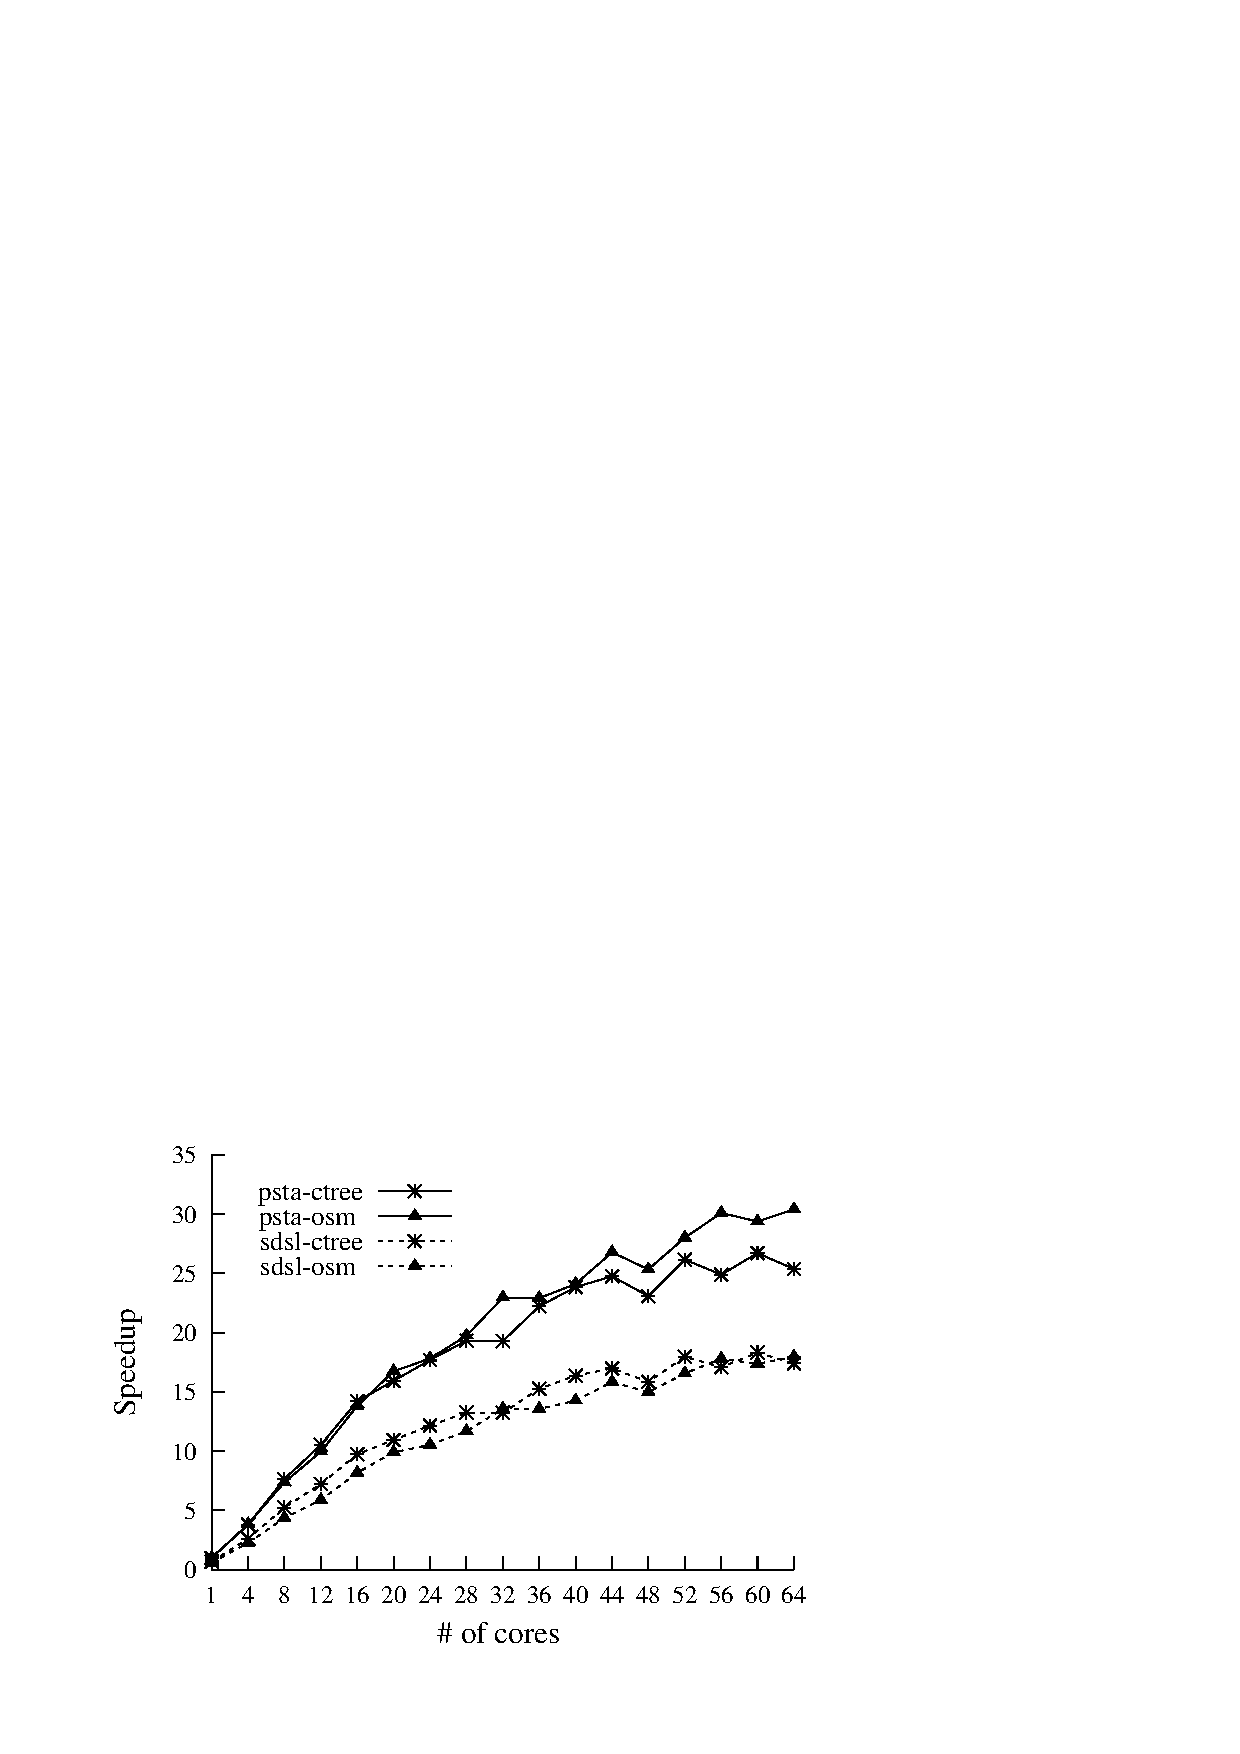
\includegraphics[width=1.04\textwidth]{./images/speedup}}
  \end{minipage}\\[1ex]
  \leavevmode\begin{minipage}[t]{0.47\textwidth}
    \captionof{table}{Running times of {\tt PSTA}, {\tt libcds}, and {\tt sdsl}
      in seconds.\label{tbl:parallelTimes}}
  \end{minipage}%
  \hspace{\stretch{1}}%
  \begin{minipage}[t]{0.5\textwidth}
    \captionof{figure}{Speed-up on {\tt ctree} and {\tt osm}
      data sets.\label{fig:speedup}}
  \end{minipage}
\end{figure}

Up to 16 cores, the speed-up of {\tt psta} is almost linear whenever $p$ is a
power of $2$ and the efficiency (speed-up/$p$) is 70\% or higher, except for
{\tt ctree} on 32 cores.
This is very good for multicore architectures.
When $p$ is not a power of~$2$, speed-up is slightly worse.
The reason is that, when $p$ is a power of $2$, {\tt psta} can assign exactly
one subtree to each thread (see Algorithm \ref{algo:PSTA2}), distributing the
work homogeneously across cores without any work stealing.
When the number of threads is not a power of two, some threads have to process
more than one subtree and other threads process only one, which degrades
performance due to the overhead of work stealing.

There were three other factors that limited the performance of {\tt psta} in
our experiments: network topology, input size, and resource contention with
the OS.

\textit{Topology.}
The four processors on our machine were connected in a grid
topology~\cite{Drepper2007}.
Up to 32 threads, all threads can be run on a single processor or on two
adjacent processors in the grid, which keeps the cost of communication between
threads low.
Beyond 32 threads, at least three processor are needed and
at least two of them are not adjacent in the grid.
This increases the cost of communication between threads on these processors
noticeably.

\textit{Input size.}
For the two largest inputs we tested, {\tt osm} and {\tt ctree}, speed-up
kept increasing as we added more cores.
For {\tt wiki}, however, the best speed-up was achieved with 36 cores.
Beyond this, the amount of work to be done per thread was small enough that
the scheduling overhead caused by additional threads started to outweigh the
benefit of reducing the processing time per thread further.

\textit{Resource contention.}
For $p < 64$, at least one core on our machine was available to OS processes,
which allowed the remaining cores to be used exclusively by {\tt psta}.
For $p = 64$, {\tt psta} competed with the OS for available cores.
This had a detrimental effect on the efficiency of {\tt psta} for $p = 64$.

\subsubsection{Memory usage.}

We measured the amount of working memory (i.e., memory not occupied by the raw
parenthesis sequence) used by {\tt psta}, {\tt libcds}, and {\tt sdsl}.
We did this by monitoring how much memory was allocated/released with
\texttt{malloc}/\texttt{free} and recording the peak usage.
For {\tt psta}, we only measured the memory usage for $p = 1$.
The extra memory needed for thread scheduling when $p > 1$ was negligible.
Due to lack of space, we report the results only for the two largest inputs,
{\tt ctree} and {\tt osm}.
For the {\tt ctree} input, {\tt psta}, {\tt libcds}, and {\tt sdsl} used 112MB,
38MB, and 76MB of memory, respectively.
For {\tt osm}, they used 331MB, 85MB, and 194MB, respectively.
Even though {\tt psta} uses more memory than both {\tt libcds} and {\tt sdsl},
the difference between {\tt psta} and {\tt sdsl} is a factor of less than two.
The difference between {\tt psta} and {\tt libcds} is no more than a factor of
four and is outweighed by the substantially worse performance of {\tt libcds}.
More importantly, 331MB for processing a 2-billion-node tree amounts to less
than one bit per node, so {\tt psta} can be considered very space-efficient.

Part of the higher memory usage of {\tt psta} stems from the allocation of
$e^{\prime}$, $m^{\prime}$, $M^{\prime}$ and $n^{\prime}$ arrays to store the
partial excess values in the algorithm.
Storing these values, however, is a key factor that helps {\tt psta} to achieve
very good performance.


\section{Conclusions and Future Work}
\label{sec:conclusion}
In this work we shown that it is possible to improve the construction time of succinct
trees, exploiting current multicore architectures. We introduce a practical algorithm that
achieves $O(n/p+\lg p)$ construction time, to a tree with $n$ nodes and $p$
threads, while supports a rich set of navigational operations in $O(\lg n)$ time. This
practical algorithm was tested against state-of-the-art libraries, reaching good speedup.
Since our algorithm needs, as input, a tree stored as a parentheses
sequence, we presented an algorithm to compute such parentheses sequence in parallel in
$O(n/p+\lg p)$ time.

In this paper we focused on static representation of succinct trees. However, our results
may be the base to the parallel construction of dynamic succinct trees, as the dynamic
succinct trees of \cite{Navarro:2014:FFS:2620785.2601073}. Also, it would be interesting
to study how to extend our results to succinct representation of \emph{labeled} trees. We
shall explore the extension of our results to the parallel construction other succinct
data structures that use succinct trees representations as part of their representations.
Such is the case of succinct planar graphs. Note that we can use the results of
\cite{Fuentes2014} to parallelize batches of navigational operations, reaching a good
pratical speedup. Since that the \emph{range min-max tree}, that our algorithms construct,
is a complete tree, the strategy underlying our algorithms can be applied to construct
general complete trees in parallel.

We believe that exploit current multicore architectures to improve the overall performance
of succinct data structures is a interesting research line. Taking the features of
succinct data structures and the processing power of multicore architectures allows to
design practical data structures with competitive querying time, efficient space usage and
fast/scalable construction time.

\subsubsection*{Acknowledgements.}
We would like to thank Diego Arroyuelo, Roberto As\'{i}n, and Rodrigo
C\'{a}novas for their time and making resources available to us.

\bibliographystyle{splncs03}
\bibliography{sigproc}

\newpage
\appendix
\begin{center}
  \bf \Large Appendices
\end{center}

\section{Operations supported by the NS-representation}
\label{sec:operations}

\begin{table}[h]
\setlength{\tabcolsep}{0pt}
\begin{center}
\begin{tabular} {l@{\hspace{1em}}>{\raggedright\arraybackslash}p{7.2cm}}
\toprule
\textbf{Operation}                 & \textbf{Description}        \\
\midrule
$\child(x,i)$                      & Find the $i$th child of node $x$\\
$\childrank(x)$                    & Report the number of left siblings of node $x$\\
$\degree(x)$                       & Report the degree of node $x$\\
$\depth(x)$                        & Report the depth of node $x$\\
$\levelanc(x,i)$                   & Find the ancestor of node $x$ that is $i$ levels above node $x$\\
$\subtreesize(x)$                  & Report the number of nodes in the subtree rooted at node $x$\\
$\height(x)$                       & Report the height of the subtree rooted at $x$\\
$\deepestnode(x)$                  & Find the deepest node in the subtree rooted at node $x$\\
$\lca(x,y)$                        & Find the lowest common ancestor of nodes $x$ and $y$ \\
$\lmostleaf(x)$ /$\rmostleaf(x)$   & Find the leftmost/rightmost leaf of the subtree rooted at node $x$\\
$\leafrank(x)$                     & Report the number of leaves before node $x$ in preorder\\
$\leafselect(i)$                   & Find the $i$th leaf from left to right\\
$\prerank(x)$/$\postrank(x)$       & Report the number of nodes preceding node $x$ in preorder/postorder\\
$\preselect$/$\postselect(i)$      & Find the $i$th node in preorder/postorder\\       
$\levellmost(i)$/$\levelrmost(i)$  & Find the leftmost/rightmost node among all nodes at depth $i$\\
$\levelsucc(x)$/$\levelpred(x)$    & Find the node immediately to the left/right of node $x$ among all nodes at depth $i$\\
\midrule
$\access(i)$                       & Report $P[i]$\\
$\findopen(i)$/$\findclose(i)$     & Find The matching parenthesis of $P[i]$\\
$\enclose(i)$                      & Find the closest enclosing matching parenthesis pair for $P[i]$\\
$\rankopen(i)$/$\rankclose(i)$     & Report the number of opening/closing parentheses in $P[1..i]$\\
$\selectopen(i)$/$\selectclose(i)$ & Find the $i$th opening/closing parenthesis\\
\bottomrule
\end{tabular}
\caption{Operations supported by the NS-representation~\cite{Navarro:2014:FFS:2620785.2601073}, including operations over the corresponding balanced parenthesis sequence.}
\label{tbl:operations}
\end{center}
\end{table}


\section{Parallel Folklore Encoding Algorithm}
\label{subsec:parenthesesAlgorithm}

\begin{algorithm}[b]
  \small
  % keywords
  \SetKwInOut{Input}{Input}
  \SetKwInOut{Output}{Output}
  \SetKwFor{PFor}{parfor}{do}{end}
  \LinesNumbered
  \DontPrintSemicolon
  \SetVlineSkip{0.5ex}
  \SetCommentSty{textit}
  % I/o
  \Input{An adjacency list representation of $T$ consisting of arrays $V$ and $E$ and the number of threads, $\threads$.}
  \Output{The balanced parenthesis sequence $P$ of $T$.}
  \BlankLine
  % algorithm
  $\id{ET} \asgn {}$an array of length $2|E|$\;
  $\id{P} \asgn {}$an array of length $2|E|+2$\;
  $\id{chk} \asgn |E|/\threads$\;
  \PFor{$t \asgn 0$ \KwTo $\threads-1$}{
    \For{$i \asgn 0$ \KwTo $\chk-1$}{
      $j \asgn t*\chk + i$\;
      $\id{ET}[2*j].\id{value} \asgn 1$ \tcp*[h]{forward edge, opening parenthesis}\;
      $\id{ET}[2*j+1].\id{value} \asgn 0$ \tcp*[h]{backward edge, closing parenthesis}\;
      \eIf{$E[j].\chld$ is a leaf}{
        $\id{ET}[2*j].\id{succ} \asgn 2*j+1$\;
      }
      {
        $\id{ET}[2*j].\id{succ} \asgn 2*\id{next}(E[j].\chld)$\;
      }
      \eIf{$E[j]$ is the last edge in the adjacency list of $E[j].\parent$}{
        $\id{ET}[2*j+1].\id{succ} \asgn 2*\id{first}(E[j].\parent)+1$\;
      }
      {
        $\id{ET}[2*j+1].\id{succ} \asgn 2*\id{next}(E[j].\parent)$\;
      }
    }
  }
  $\id{parallel\_list\_ranking}(\id{ET})$\;
  \PFor{$t \asgn 0$ \KwTo $\threads - 1$}{
    \For{$i \asgn 0$ \KwTo $2*\chk-1$}{
      $P[\id{ET}[2*t*\chk+i+1].\id{rank}] \asgn \id{ET}[2*t*\chk+i+1].\id{value}$\;
    }
  }
  $P[0] \asgn 1$\;
  $P[2|E|+1] \asgn 0$\;
  \vspace{1ex}
  \caption{{\tt PFEA}}
  \label{algo:PFEA}
  \end{algorithm}

The {\tt PSTA} algorithm requires the input tree $T$ to be given in the form
of a balanced parenthesis sequence $P$, but in many applications $T$ may not
be given in this form.
Here, we present a parallel algorithm that constructs the balanced parenthesis
sequence of $T$ from a representation of $T$ stored in adjacency list
representation.
Since the balanced parenthesis sequence of $T$ is also known as its
``folklore encoding'', we call the algorithm the
\emph{Parallel Folklore Encoding Algorithm} ({\tt PFEA}).
The input tree is represented by an array of nodes, $V$, and an array of edges,
$E$.
Each node $v$ in $V$ stores a pointer to an adjacency list with one entry per
edge incident to $v$, sorted counterclockwise around $v$, starting with $v$'s
parent edge.
Each entry in this adjacency list points to $v$ and to the edge in $E$ it
represents.
Each edge $e=(u,v)$ in $E$ points to its corresponding entries in the adjacency
lists of $u$ and $v$.
Edges are assumed to be directed from parents to children.
Thus, for an edge $e = (u, v)$, we refer to $u$ and $v$ as $e.\parent$ and
$e.\chld$, respectively.
For $x \in \{u, v\}$, we use $\id{next}(e.x)$ and $\id{first}(e.x)$ to denote
the indices in $E$ of $e$'s successor and of the first element in $x$'s
adjacency list, respectively.
Both are easily computed in constant time by following pointers.

The idea behind the construction is the following: Given an Euler tour of $T$
that visits the children of each node in left-to-right order, then the balanced
parenthesis representation of $T$ can be obtained by following the Euler tour,
writing down an opening parenthesis for every edge traversed from parent to child
and a closing parenthesis for every edge traversed from child to parent, and
finally enclosing the resulting sequence in a pair of parentheses representing
the root of $T$.

Algorithm~\ref{algo:PFEA} shows the pseudo-code of the construction.
It creates two arrays, one an auxiliary array $\id{ET}$ of length $2|E|$ to
store the Euler tour of $T$, the other an array $P$ of size $2|E|+2$ to store
the balanced parenthesis representation of $T$ (lines 1--2).
Each entry in $\id{ET}$ represents the traversal of an edge of $T$ and stores
three values: $\id{value}$ is ``(`` or ``)'' depending on whether the edge is
traversed from parent to child or from child to parent, that is, it's the
corresponding parenthesis to be added to $P$; $\id{succ}$ is the index in
$\id{ET}$ of the next edge in the Euler tour; and $\id{rank}$ is the rank in
the Euler tour.
Lines~4--16 of the algorithm populate $\id{ET}$ with entries representing
the Euler tour but leaving the $\id{rank}$ values uninitialized.
Line~17 computes ranks using a parallel list ranking algorithm~\cite{Helman2001265}.
Given these ranks, the balanced parenthesis representation can be obtained by
writing $\id{ET}[i].\id{value}$ into $P[\id{ET}[i].\id{rank}]$.
Lines~18--22 do exactly this.

Lines~4--16 and 18--22 perform $O(n)$ work and have span $O(n/p)$.
The whole computation here (and in Lines~18--22) could have been formulated as a
single parallel loop.
However, in the interest of limiting scheduling overhead, we create only as many
parallel threads as necessary, similar to the {\tt PSTA} algorithm in
Section~\ref{sec:multicoreST}.
Line~17 performs $O(n)$ work and has span $O(\lg p + n/p)$.
This gives a total work of $T_1 = O(n)$ and a span of $T_\infty = O(\lg n)$.
The running time on $p$ cores is $T_p = O(n/p + \lg p)$.


\end{document}

